% Figure snippets for the ELD manuscript.
% These are intended to be embedded inline by the writing agent, not \input'd.

\begin{figure}[htbp]
\centering

\includegraphics[width=0.95\textwidth]{figures/fig_pipeline.pdf}
\caption{End-to-end ELD pipeline. Two tissue sections (Visium, H\&E, ISS, or MSI) are fed into the hourglass landmark detector (or, optionally, are replaced by manual annotation), landmarks drive a thin-plate spline (or homography) registrar, and the registered sections are projected into a common coordinate framework that supports cross-section comparison.}
\label{fig:pipeline}
\end{figure}

\begin{figure}[htbp]
\centering
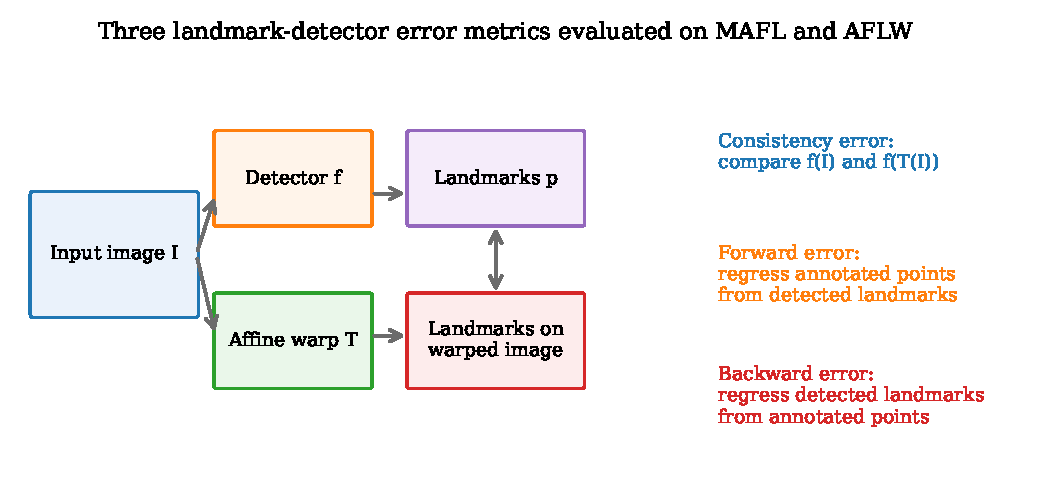
\includegraphics[width=0.88\textwidth]{figures/fig_errors.pdf}
\caption{Schematic of the three landmark-detector error metrics adopted from~\cite{sanchez2019object}. Consistency error measures geometric self-agreement under affine warps; forward error measures how well detected landmarks predict manual annotations via linear regression; backward error measures the reverse prediction and captures landmark stability.}
\label{fig:errors}
\end{figure}

\begin{figure}[htbp]
\centering
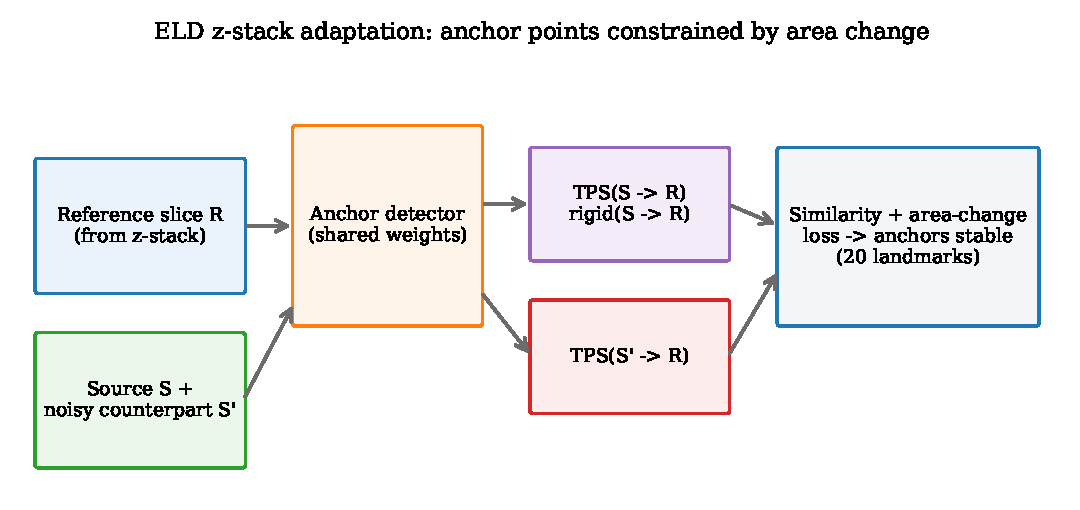
\includegraphics[width=0.95\textwidth]{figures/fig_3d_workflow.pdf}
\caption{Z-stack adaptation of ELD. A reference slice is selected at random from the stack; a source slice and a noisy counterpart are each passed through the landmark detector; the similarity loss between the noisy and clean source mappings is combined with the area-change difference between TPS and rigid maps, forcing landmarks to behave as anchor points with fixed x-y coordinates.}
\label{fig:3d_workflow}
\end{figure}

\begin{figure}[htbp]
\centering
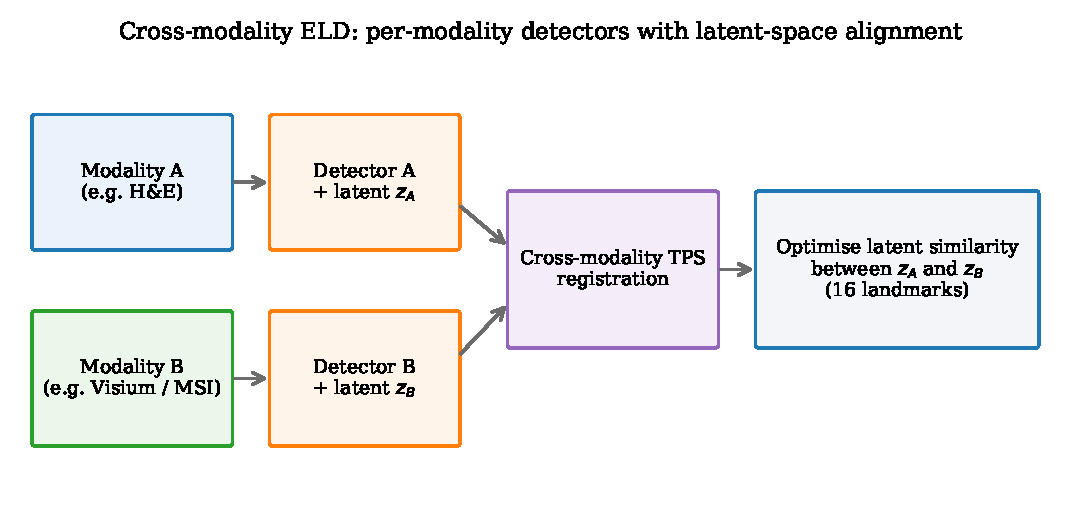
\includegraphics[width=0.95\textwidth]{figures/fig_multimodal_workflow.pdf}
\caption{Cross-modality ELD architecture. Two modality-specific hourglass detectors produce landmarks and latent representations for modality A (e.g.\ H\&E) and modality B (e.g.\ Visium or MSI). Samples are registered with TPS guided by the detected landmarks, and the similarity of the two modalities' latent representations is optimised jointly.}
\label{fig:multimodal_workflow}
\end{figure}
